\documentclass[epsfig,10pt,fullpage]{article}

\newcommand{\LabNum}{8}
\newcommand{\CommonDocsPath}{../../common/docs}
\addtolength{\textwidth}{1.5in}
\addtolength{\oddsidemargin}{-0.75in}
\addtolength{\topmargin}{-0.75in}
\addtolength{\textheight}{1.5in}
\addtolength{\evensidemargin}{0.75in}
\setlength\parindent{0pt}
\raggedbottom

\usepackage{ae,aecompl}
\usepackage{epsfig,float,times}
\usepackage[hypcap]{caption}
\usepackage[pdftex, colorlinks]{hyperref}
\usepackage{graphicx}
\usepackage[usenames, dvipsnames]{color}
\usepackage{rotating}
\usepackage{tikz}
\usetikzlibrary{automata,positioning}
\usepackage{placeins}

\widowpenalty 10000
\clubpenalty 10000

\newcommand{\red}[1]{{\color{red}\sf{#1}}}
\newcommand{\green}[1]{{\color{green}\sf{#1}}}
\newcommand{\blue}[1]{{\color{blue}\sf{#1}}}
\definecolor{PineGreen}{rgb}{0.0, 0.47, 0.44}
\definecolor{ForestGreen}{rgb}{0.13, 0.55, 0.13}
\definecolor{Brown}{rgb}{0.59, 0.29, 0.0}

\newcommand{\UPDatePublished}{Oct 2021}
\newcommand{\versnum}{21.1} %version number quartus/AMP
\newcommand{\quartusname}{Quartus\textsuperscript{\textregistered} Prime}	
\newcommand{\UPTextBar}{For \quartusname{} \versnum{}}
\newcommand{\thisyear}{2021 } %for copyright
\newcommand{\company}{FPGAcademy.org}
\newcommand{\longteamname}{FPGAcademy.org}
\newcommand{\teamname}{FPGAcademy}
\newcommand{\website}{FPGAcademy.org}

\newcommand{\productAcronym}{AMP}
\newcommand{\productNameShort}{Monitor Program}

\newcommand{\productNameMedTM}{A Monitor Program}
\newcommand{\productNameMed}{A Monitor Program}

%\newcommand{\headerLogoFilePath}[1]{#1/FPGAcademy.png}

% listings is a package that supports encapsulating source code in LaTeX conveniently
\usepackage{listings}

\def\expandparam\lstinputlisting[#1]#2{\edef\tmp{\noexpand\lstinputlisting[#1]{#2}}\tmp}

%%%%%%%%%%%%%%%%%%%% Source Code Formatting %%%%%%%%%%%%%%%%%%%%
\definecolor{globalCommentColour}{rgb}{0.588,0.588,0.588}

%%%%%%%%%%%%%%%%%%%%%%%%%%%%%%%%%%%%%%%%%%%%%%%%%%%%
% Defining language style
% NiosII ASM
\lstdefinelanguage[NiosII]{Assembler} {
  morekeywords={add, addi, and, andhi, andi, beq, bge, bgeu, bgt, bgtu, ble,  bleu, blt, bltu, bne, br, break,
  bret, call, callr, cmpeq, cmpeqi, cmpge, cmpgei, cmpgeu, cmpgeui, cmpgt, cmpgti, cmpgtu, cmpgtui, cmple,
  cmplei, cmpleu, cmpleui, cmplt, cmplti, cmpltu, cmpltui, cmpne, cmpnei, custom, div, divu, eret, flushd,
  flushda, flushi, flushp, initd, initda, initi, jmp, jmpi, ldb, ldbio, ldbu, ldbuio, ldh, ldhio, ldhu, ldhuio,
  ldw, ldwio, mov, movhi, movi, movia, movui, mul, muli, mulxss, mulxsu, mulxuu, nextpc, nop, nor, or, orhi, ori,
  rdctl, rdprs, ret, rol, roli, ror, sll, slli, sra, srai, srl, srli, stb, stbio, sth, sthio, stw, stwio,
  sub, subi, sync, trap, wrctl, wrtcl, wrprs, xor, xori, xorhi, xori},
  morekeywords=[2]{.abort, .ABORT, .align, .app-file, .ascii, .asciz, .balign, .byte, .comm, .data, .def,
  .desc, .dim, .double, .eject, .else, .end, .endef, .endif, .equ, .equiv, .err, .extern, .file, .fill, .float,
  .global, .globl, .hword, .ident, .if, .include, .int, .irp, .irpc, .lcomm, .lflags, .line, .linkonce, .ln,
  .list, .long, .macro, .mri, .nolist, .octa, .org, .p2align, .psize, .quad, .rept, .sbttl, .scl, .section,
  .set, .short, .single, .size, .sleb128, .skip, .space, .stadb, .stabn, .stabs, .string, .symver, .tag,
  .text, .title, .type, .val, .uleb128, .word},
  morekeywords=[3]{et, bt, gp, sp, fp, ea, sstatus, ra, pc, status, estatus, bstatus, ienable, ipending, cpuid,
  exception, pteaddr, tlbacc, tlbmisc, eccinj, badaddr, config, mpubase, mpuacc},
  sensitive=t,
  alsoletter=.,
  morestring=[b]",
  morecomment=[s]{/*}{*/},
  morecomment=[l]\#,
}[keywords,comments,strings]
   
%% NOTE: morekeywords=[2] are GNU directives.
   
\definecolor{niosInstructionColour}{rgb}{0.000,0.608,0.000}
\definecolor{niosDirectiveColour}{rgb}{0.000,0.000,0.902}
\definecolor{niosSpecialRegColour}{rgb}{0.000,0.000,0.000}
\definecolor{niosStringColour}{rgb}{0.808,0.482,0.000}
   
%% NOTE: To make bold use: =\bfseries\color{<colour>}
\lstdefinestyle{defaultNiosStyle} {
  language=[NiosII]{Assembler},
  stringstyle=\color{niosStringColour},
  keywordstyle=\color{niosInstructionColour},
  keywordstyle=[2]\color{niosDirectiveColour},
  keywordstyle=[3]\itshape\color{niosSpecialRegColour}
}
%%%%%%%%%%%%%%%%%%%%%%%%%%%%%%%%%%%%%%%%%%%%%%%%%%%%

%%%%%%%%%%%%%%%%%%%%%%%%%%%%%%%%%%%%%%%%%%%%%%%%%%%%
% Defining language style
% ArmA9 ASM
\lstdefinelanguage[ArmA9]{Assembler} {
  morekeywords={ADC, ADD, ADDS, AND, ANDS, B, BAL, BEQ, BGE, BGT, BL, BLT, BIC, BKPT, BLX, BNE, BX, CDP, CLZ, CMN, CMP, EOR,
  EORS, LDC, LDM, LDR, LDRB, LDRBT, LDRH, LDRSB, LDRSH, LDRT, LSL, MCR, MLA, MOV, MOVW, MOVT, MRC, MRS, MSR, MUL, MVN, ORR, PLD,
  ROR, RSB, RSC, SBC, SMLAL, SMULL, STC, STM, STR, STRB, STRBT, STRH, STRT, SUB, SUBS, SWI, SWP, SWPB, TEQ, UMLAL,
  PUSH, POP, MOVS, RORS, LSR},
  morekeywords=[2]{.abort, .ABORT, .align, .app-file, .ascii, .asciz, .balign, .byte, .comm, .data, .def,
  .desc, .dim, .double, .eject, .else, .end, .endef, .endif, .equ, .equiv, .err, .extern, .file, .fill, .float,
  .global, .globl, .hword, .ident, .if, .include, .int, .irp, .irpc, .lcomm, .lflags, .line, .linkonce, .ln,
  .list, .long, .macro, .mri, .nolist, .octa, .org, .p2align, .psize, .quad, .rept, .sbttl, .scl, .section,
  .set, .short, .single, .size, .sleb128, .skip, .space, .stadb, .stabn, .stabs, .string, .symver, .tag,
  .text, .title, .type, .val, .vectors, .uleb128, .word},
  morekeywords=[3]{SP, PC, MIDR, CTR, TCMTR, TLBTR, MPIDR, ID_PFR0, ID_PFR1, ID_DFR0, ID_MMFR0, ID_MMFR1, ID_MMFR2,
  ID_MMFR3, ID_ISAR0, ID_ISAR1, ID_ISAR2, ID_ISAR3, ID_ISAR4, CCSIDR, CLIDR, AIDR, CSSELR, TTBR0, TTRB1, TTBR2, DACR,
  DFSR, IFSR, ADFSR, AIFSR, DFAAR, IFAR, ICIALLUIS, BPIALLIS, PAR, ICIALLU, ICIMVAU, BPIALL, DCIMVAC, DCISW, V2PCWPR,
  DCCVAC, DCCSW, DDIMVAC, DCISW, TLBALLIS, TLBIMVAIS, TLBIASIDIS, TLBIMVAAIS, TLBIALL, TLBIMVA, TLBIASID, TLBIMVAA,
  PMCR, PMCNTENSET, PMCNTENCLR, PMOVSR, PMSWINC, PMSELR, PMXEVTYPER, PMXEVCNTR, PMUSERENR, PMINTENSET, PMINTENCLR,
  PRRR, NRRR, PLEIDR, PLEASR, PLEFSR, PLEUAR, PLEPCR, VBAR, MVBAR, ISR, FCSEIDR, CONTEXTIDR, TPIDRURW, TPIDRURO, TPIDRPRW},
  sensitive=f,
  alsoletter=.,
  morestring=[b]",
  morecomment=[s]{/*}{*/},
  morecomment=[l]{//},
}[keywords,comments,strings]
   
%% NOTE: morekeywords=[2] are GNU directives.
   
\definecolor{armInstructionColour}{rgb}{0.000,0.608,0.000}
\definecolor{armDirectiveColour}{rgb}{0.000,0.000,0.902}
\definecolor{armSpecialRegColour}{rgb}{0.000,0.000,0.000}
\definecolor{armStringColour}{rgb}{0.808,0.482,0.000}
   
\lstdefinestyle{defaultArmStyle} {
  language=[ArmA9]{Assembler},
  stringstyle=\color{armStringColour},
  keywordstyle=\color{armInstructionColour},
  keywordstyle=[2]\color{armDirectiveColour},
  keywordstyle=[3]\itshape\color{armSpecialRegColour}
}
%%%%%%%%%%%%%%%%%%%%%%%%%%%%%%%%%%%%%%%%%%%%%%%%%%%%

%%%%%%%%%%%%%%%%%%%%%%%%%%%%%%%%%%%%%%%%%%%%%%%%%%%%
% Defining language style
% FPGAcademy ASM
\lstdefinelanguage{ASM}{
  morekeywords = [1]{mv, mvt, mvne, mvcc, add, sub, st, ld, and, b, bne, beq, bcc, bcs},
  morekeywords = [2]{word, define},
  keywordstyle = [1]\color{ForestGreen},
  keywordstyle = [2]\color{blue},
  sensitive = true,
  morecomment = [l]{//},
}

\lstset{
  language = ASM,
  basicstyle=\small\color{black}\ttfamily,
  commentstyle=\small\color{Brown}\itshape\ttfamily,
  showstringspaces=false,
  frame=none, %lines % boxed listings
  breaklines=true,
  breakatwhitespace=true,
  tabsize=3
}
%%%%%%%%%%%%%%%%%%%%%%%%%%%%%%%%%%%%%%%%%%%%%%%%%%%%

%%%%%%%%%%%%%%%%%%%%%%%%%%%%%%%%%%%%%%%%%%%%%%%%%%%%
% Defining language style
% Java
\definecolor{javaStringColour}{rgb}{0.808,0.482,0}
%%%%%%%%%%%%%%%%%%%%%%%%%%%%%%%%%%%%%%%%%%%%%%%%%%%%

%%%%%%%%%%%%%%%%%%%%%%%%%%%%%%%%%%%%%%%%%%%%%%%%%%%%
% Defining language style
% C
\definecolor{CStringColour}{rgb}{0.808,0.482,0}

\lstset{
  language = C,
  basicstyle=\small\color{black}\ttfamily, 
  commentstyle=\small\color{PineGreen}\itshape\ttfamily,
  keywordstyle=\small\color{blue}\bfseries\ttfamily,
  showstringspaces=false,
  frame=none, %lines % boxed listings
  breaklines=true,
  breakatwhitespace=true,
  tabsize=3
}
%%%%%%%%%%%%%%%%%%%%%%%%%%%%%%%%%%%%%%%%%%%%%%%%%%%%

%%%%%%%%%%%%%%%%%%%%%%%%%%%%%%%%%%%%%%%%%%%%%%%%%%%%
% Defining language style
% Verilog
\definecolor{verilogCommentColour}{rgb}{0.000,0.502,0.000}

\lstdefinestyle{defaultVerilogStyle} {
  language={Verilog},
  keywordstyle=\color{blue},
  commentstyle=\color{verilogCommentColour}
}
%%%%%%%%%%%%%%%%%%%%%%%%%%%%%%%%%%%%%%%%%%%%%%%%%%%%

%%%%%%%%%%%%%%%%%%%%%%%%%%%%%%%%%%%%%%%%%%%%%%%%%%%%
% Defining language style
% VHDL
\lstdefinestyle{defaultVHDLStyle} {
  language={VHDL},
  keywordstyle=\color{blue},
  commentstyle=\color{verilogCommentColour}
}
%%%%%%%%%%%%%%%%%%%%%%%%%%%%%%%%%%%%%%%%%%%%%%%%%%%%

%%%%%%%%%%%%%%%%%%%%%%%%%%%%%%%%%%%%%%%%%%%%%%%%%%%%
% Defining language style
% LaTeX
\lstdefinelanguage[LocalLaTeX]{TeX}[LaTeX]{TeX}{moretexcs={bf, it, sf, lstset},}

\lstdefinestyle{defaultLocalLatexStyle} {
  language=[LocalLatex]{TeX},
  keywordstyle=\color{blue}\bfseries,
  keywordstyle=[2]\color{blue},
  keywordstyle=[3]\color{blue}\bfseries
}
%%%%%%%%%%%%%%%%%%%%%%%%%%%%%%%%%%%%%%%%%%%%%%%%%%%%

%%%%%%%%%%%%%%%%%%%%%%%%%%%%%%%%%%%%%%%%%%%%%%%%%%%%
% Defining language style
% Default
\lstset{
  basicstyle=\small\color{black}\ttfamily,
  commentstyle=\small\color{globalCommentColour}\itshape\ttfamily,
  keywordstyle=\small\color{blue}\bfseries\ttfamily,
  showstringspaces=false,
  frame=none, %lines % boxed listings
  breaklines=true,
  breakatwhitespace=true,
  tabsize=3
}
%%%%%%%%%%%%%%%%%%%%%%%%%%%%%%%%%%%%%%%%%%%%%%%%%%%%


\hypersetup{
  pdftitle={Embedded Systems Lab Exercise \LabNum},
  linkcolor=blue,
  hyperindex=true,
  pdfauthor={FPGAcademy.org},
  pdfkeywords={FPGAcademy.org, FPGAcademy, Lab, Exercise, Embedded Systems},
  bookmarks,
  bookmarksopen=false,
  filecolor=blue,
  pdfstartview={FitH},
  urlcolor=blue,
  plainpages=false,
  pdfpagelabels=true,
  linkbordercolor={1 1 1} %no color for link border
}



\begin{document}

\centerline{\huge Embedded Systems}
~\\
\centerline{\huge Laboratory Exercise \LabNum}
~\\
\centerline{\large Audio and an Introduction to Multithreaded Applications}
~\\

\noindent
The purpose of this exercise is to create user-level Linux* programs that 
produce audio output on a DE-series board. The final application task for this exercise is
to implement a digital piano that can play musical chords through the audio port of the board.
In addition to listening to the music, you will also be able to visualize the sound as
waveforms on a display, and record/playback tones. As part of this exercise, you will also
be introduced to writing {\it multithreaded} applications.

~\\
\noindent
{\bf Using the Audio Port}

~\\
\noindent
Several DE-series boards provide audio input/output capability via an audio CODEC (COder/DECoder) 
chip. In the discussion below we assume that the reader is using the DE1-SoC board. If 
a different board, such as the DE10-Standard or DE10-Nano, is being used the same instructions 
can usually be followed, with some modifications.

~\\
\noindent
The DE1-SoC Computer includes an audio port that is connected to the audio CODEC chip. 
Audio output capability is provided via the line-out jack (3.5 mm green connector), and 
audio input via the microphone jack (pink connector).
For this exercise you will use only the audio output feature. The audio port includes 
two {\it Write} FIFOs (queues) that are used to hold outgoing data, as well as two {\it Read}
FIFOs (not used here) for incoming data. These FIFOs have a maximum depth of 128 32-bit words.
If the sampling rate of the audio port is 8000 samples/second, then a sample is removed 
from the {\it Write} FIFOs and converted to an analog voltage on the line-out jack each 
8000$^{th}$ of a second.

~\\
\noindent
The audio port's programming interface consists of four 32-bit registers, as illustrated in 
Figure \ref{fig:audio_port}. The {\it Control} register, which has the address {\sf 0xFF203040},
is readable to provide status information and writable to make control settings. Bits {\it RE}
and {\it WE} are available for enabling the generation of processor interrupts from the
audio port; you should set these bits to 0, as we are not using interrupts in this exercise.
The bit {\it CW} can be set to 1 to clear the {\it Write} FIFO. The clear function remains
active until {\it CW} is set back to 0. The read-only {\it Fifospace} register contains four
8-bit fields. The fields {\it WSRC} and {\it WSLC} give the number of words currently available
for storing data in the right and left audio-out FIFOs. When the FIFOs are empty, the values
are {\it WSRC} $=$ {\it WSLC} $=$ 128. The {\it Leftdata} and {\it Rightdata} registers
are writable for audio out. When data is written into these registers it is loaded into the 
{\it Write} FIFOs.

\begin{figure}[H]
   \begin{center}
       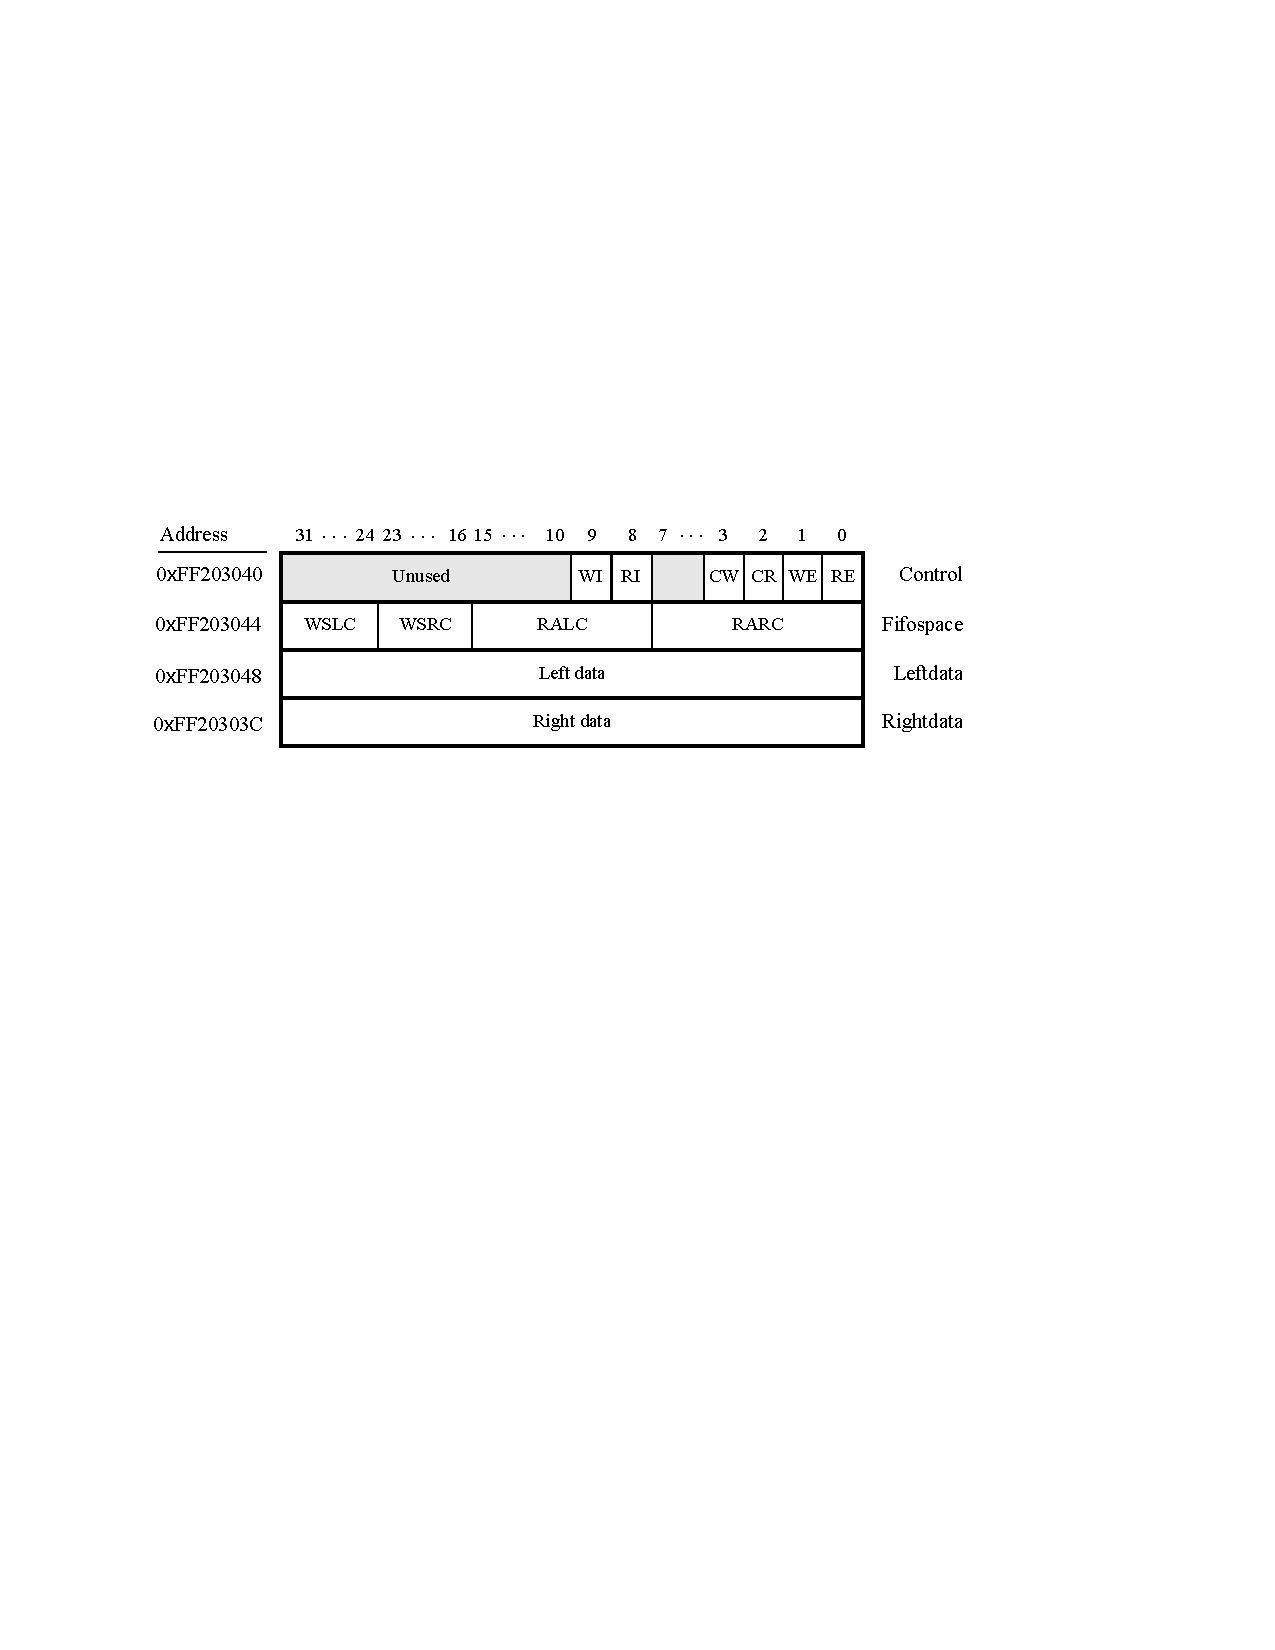
\includegraphics{figures/fig_audio_port.pdf}
   \end{center}
   \caption{Audio port registers.}
	\label{fig:audio_port}
\end{figure}

\noindent
\section*{Part I}

\noindent
You are to write a program that plays the tones of the middle C chromatic scale
through the audio-out port
of the DE1-SoC Computer system. The tones and their respective frequencies are shown in
Table~\ref{tab:tone_freqs}. When executed, your program should play these tones in sequence
from the low C (261.63~Hz) to the higher C (523.25~Hz), then terminate. The tones should be
outputted as sinusoidal waves, with each tone lasting 300 ms.

\begin{table}[H]
    \begin{center}
    \begin{tabular}{l|c}
            \textbf{Note} &
            \textbf{Frequency (Hz)}
				\\\hline\vspace{-3mm}\\
            C & 261.626 \\
            C\#/Db & 277.183 \\
            D & 293.665 \\
            D\#/Eb & 311.127 \\
            E & 329.628 \\
            F & 349.228 \\
            F\#/Gb & 369.994 \\
            G & 391.995 \\
            G\#/Ab & 415.305 \\
            A & 440.000 \\
            A\#/Bb & 466.164 \\
            B & 493.883 \\
            C & 523.251 \\

    \end{tabular}
    \caption{Notes of the middle C chromatic scale and their frequencies.}
	 \label{tab:tone_freqs}
    \end{center}
\end{table}

~\\
\noindent
Perform the following:

\begin{enumerate}
\item Make a new folder to hold your C source code. Write a file {\it part1.c} for your
\texttt{main} function, and any other source-code files that you require. To communicate
with the audio port use the memory-mapped I/O addresses given in Figure \ref{fig:audio_port}.
You will need to {\it map} the physical addresses of the audio port into virtual addresses
by using Linux kernel functions like {\it mmap} and the {\it /dev/mem} interface.
These concepts are discussed in detail in the tutorial {\it Using Linux on DE-series Boards}.
To initialize the audio port you first should clear the {\it Write} FIFO by using the {\it CW} 
bit in the {\it Control} register. 

To output a sinusoidal wave to the audio port, use the $\sin(x)$ function provided by the
library \texttt{<math.h>}. The code shown in Figure~\ref{fig:sinusoid_code}
demonstrates its use to output a 261.63~Hz tone (the middle C). To compile
C code that uses the \texttt{<math.h>} library, you must append \texttt{-lm} to the end of your
\texttt{gcc} command. The \texttt{-lm} flag instructs the compiler to include the math library
as part of your program. Since the {\it sin} function uses radians to measure the {\it phase},
you will need to calculate the number of radians per sample for each tone, and then use a
loop to output 300 ms of samples for each tone. Each audio sample is a 32-bit signed integer. 
You can produce an integer sample by multiplying the output of the {\it sin} function, 
which is a real number between -1.0 and 1.0, by the value \texttt{0x7FFFFFFF}. The audio
device sampling rate is 8,000 samples per second for the DE1-SoC and DE10-Standard boards,
and 12,000 samples per second for the DE10-Nano.
\item Connect headphones or a speaker to the audio-out jack (3.5 mm green connector) on the
DE1-SoC board. Compile your program using a command such as \texttt{gcc -o part1 part1.c -lm}, 
and then run the program to hear the tones. If you are using the DE10-Nano board then
audio output is not available via an audio jack---on this board audio can only be accessed via 
the HDMI connector that provides video output. To hear the audio you can connect the HDMI port 
to a video terminal that has audio output capability. Alternatively, you can save the
audio samples that are written to the audio device to a file and then playback that file
on a host computer. Code for creating a Microsoft* Windows* {\it WAV} file, with 16-bit signed
data, is provided along with this exercise.
\end{enumerate}

\noindent
\section*{Part II}

\noindent
In Part I you wrote a program that is capable of playing a single tone at a time. Now you will
write a program that is capable of playing multiple tones simultaneously (chords). Your program
should accept a single command-line input string of 13 '1's and '0's, 
which turn on and off the 13 tones
of the chromatic scale. For example, running your program with \texttt{./part2 1000100100000}
should play the notes C (261.63~Hz), E, and G. Your program should play the selected tones
simultaneously for one second, and then terminate. 

~\\
\noindent
To output multiple tones simultaneously, you will have to generate samples that are a sum of
multiple sinusoids. When doing so, you must be careful of possible overflows; the sum of multiple
sinusoid samples should not overflow a signed 32-bit value. One solution is to set 
each tone's maximum volume to be the value \texttt{0x7FFFFFFF} volume divided by 13, which ensures 
that the maximum possible value (when all 13 tones are being played) does not exceed the limit. 

\lstset{language=C,numbers=left,escapechar=|}
\begin{figure}[H]
\begin{center}
\begin{minipage}[t]{14.75 cm}
\begin{lstlisting}
#include <math.h>

#define 2PI 6.28318531
#define SAMPLE_RATE 8000
|$\ldots$|
int main(void){
	int nth_sample;
	double freq = 261.626;
	// Max volume, which is later multiplied by sin() (which ranges from -1 to 1)
	int vol = 0x7FFFFFFF; 

	// Write 8000 samples (one second's worth) of middle C (261.63~Hz)
	for (nth_sample = 0; nth_sample < |$\ldots$|; nth_sample++){
		write_to_audio_port(vol * sin(nth_sample * <some math goes here>));
	}
}
\end{lstlisting}
\end{minipage}
\end{center}
\vspace{-0.33in}\caption{Using the $sin$ function to make samples for middle C (261.63~Hz).}
\label{fig:sinusoid_code}
\end{figure}

~\\
\noindent
Perform the following:

\begin{enumerate}
\item Make a new folder to hold your C source code. Augment your code from Part I to create a
new file {\it part2.c}, in which the main program accepts one 13-character {\it string} argument.
Create an integer array such as \texttt{int tone\_volumes[13]} to store the volume for
each tone, based the command-line argument of your program. Use a loop to create your
sinusoidal waveform in which each sample is the sum of individual tones, for a duration of one
second.
\item Compile your program using a command such as \texttt{gcc -o part2 part2.c -lm}, 
and then run the program to verify that each tone, and chords, are played properly.
\end{enumerate}

\noindent
\section*{Part III}

In this part you will extend your code from Part II to create a simple digital piano. You
will make use of the concept of {\it threads} to create a {\it multithreaded} program, as
discussed below. 

~\\
\noindent
{\bf Introduction to Multithreaded Applications}

~\\
\noindent
A {\it thread} refers to an independent sequence of instructions executed by a processor. An 
application program can run as a single thread, or as multiple threads. When there are multiple
threads running concurrently, it is the job of the operating system (Linux) to schedule 
the threads for execution. In this way the CPU core(s) of your computer can be shared among the 
threads of your program(s).

~\\
\noindent
When running on a computer with multiple {\it CPU cores}, breaking up a program into
multiple threads allows parts of the program to run in parallel, on the multiple CPU cores.
The possible benefits of multithreading include higher throughput and lower latency. 
In this part of the exercise we will explore how to use C-code to write a
multithreaded program. This implementation will
help to ensure that a CPU core is always available to fill the {\it Write} FIFOs of the
audio port, so that there are no ``empty spaces'' in the sounds being played, and at the
same time another CPU core is available to process user inputs. 

~\\
\noindent
The digital piano will have two continuous tasks. The first is to listen for user input 
and set the \texttt{tone\_volume} array based on which tones are to be played. The second is
to constantly write samples to the audio port. While it would be possible to
have a single thread that does both
tasks by interleaving them, doing so would have drawbacks. First, it could be detrimental to
your program's responsiveness to user inputs as your program must write to the audio port in
between reads of the keyboard. Likewise, since your program would have to interleave reads
of the keyboard with writes to the audio port, the program may sometimes fail 
to supply the port with a
sample every 1/8000 seconds. Having two threads solves these issues by doing both tasks
simultaneously on the dual-core ARM* processor of the DE1-SoC computer.

~\\
\noindent 
Your program should have two threads: the {\it main thread}, which is responsible 
for listening to user input, and the {\it audio thread}, which is responsible for writing 
samples to the audio port.
The main thread is created when your program is first executed (starting from
\texttt{main($\ldots$)}).
To provide piano ``keys'' you will connect a USB keyboard to the DE1-SoC board, following the
mappings shown in Figure~\ref{fig:keyboard_layout}. The keyboard can be plugged into any
USB port on the DE1-SoC board, and will be automatically recognized by the Linux system.
Wireless keyboards can also be used, by plugging the transmitter/receiver for the keyboard
into a USB port on the DE1-SoC board. If you are using the DE10-Nano board, then
an adaptor is needed to connect the {\it USB type-A} connector of the keyboard to the 
{\it micro-USB} port that is available on the DE10-Nano board. 

~\\
\noindent
Once a keyboard is plugged in, Linux provides access to it via a device file located in
\textit{/dev/input/}. For example, a keyboard plugged into the board might be represented by
the device file \textit{/dev/input/by-id/generic-brand-USKeyboard-event-kbd}. 
Figure~\ref{fig:keyboard_code} shows C-language code that opens a keyboard device file and
listens for user key strokes. Information about using a keyboard in this way can be found
on the Internet by searching for keywords such as ``Linux event device keyboard''.

\begin{figure}[H]
   \begin{center}
			  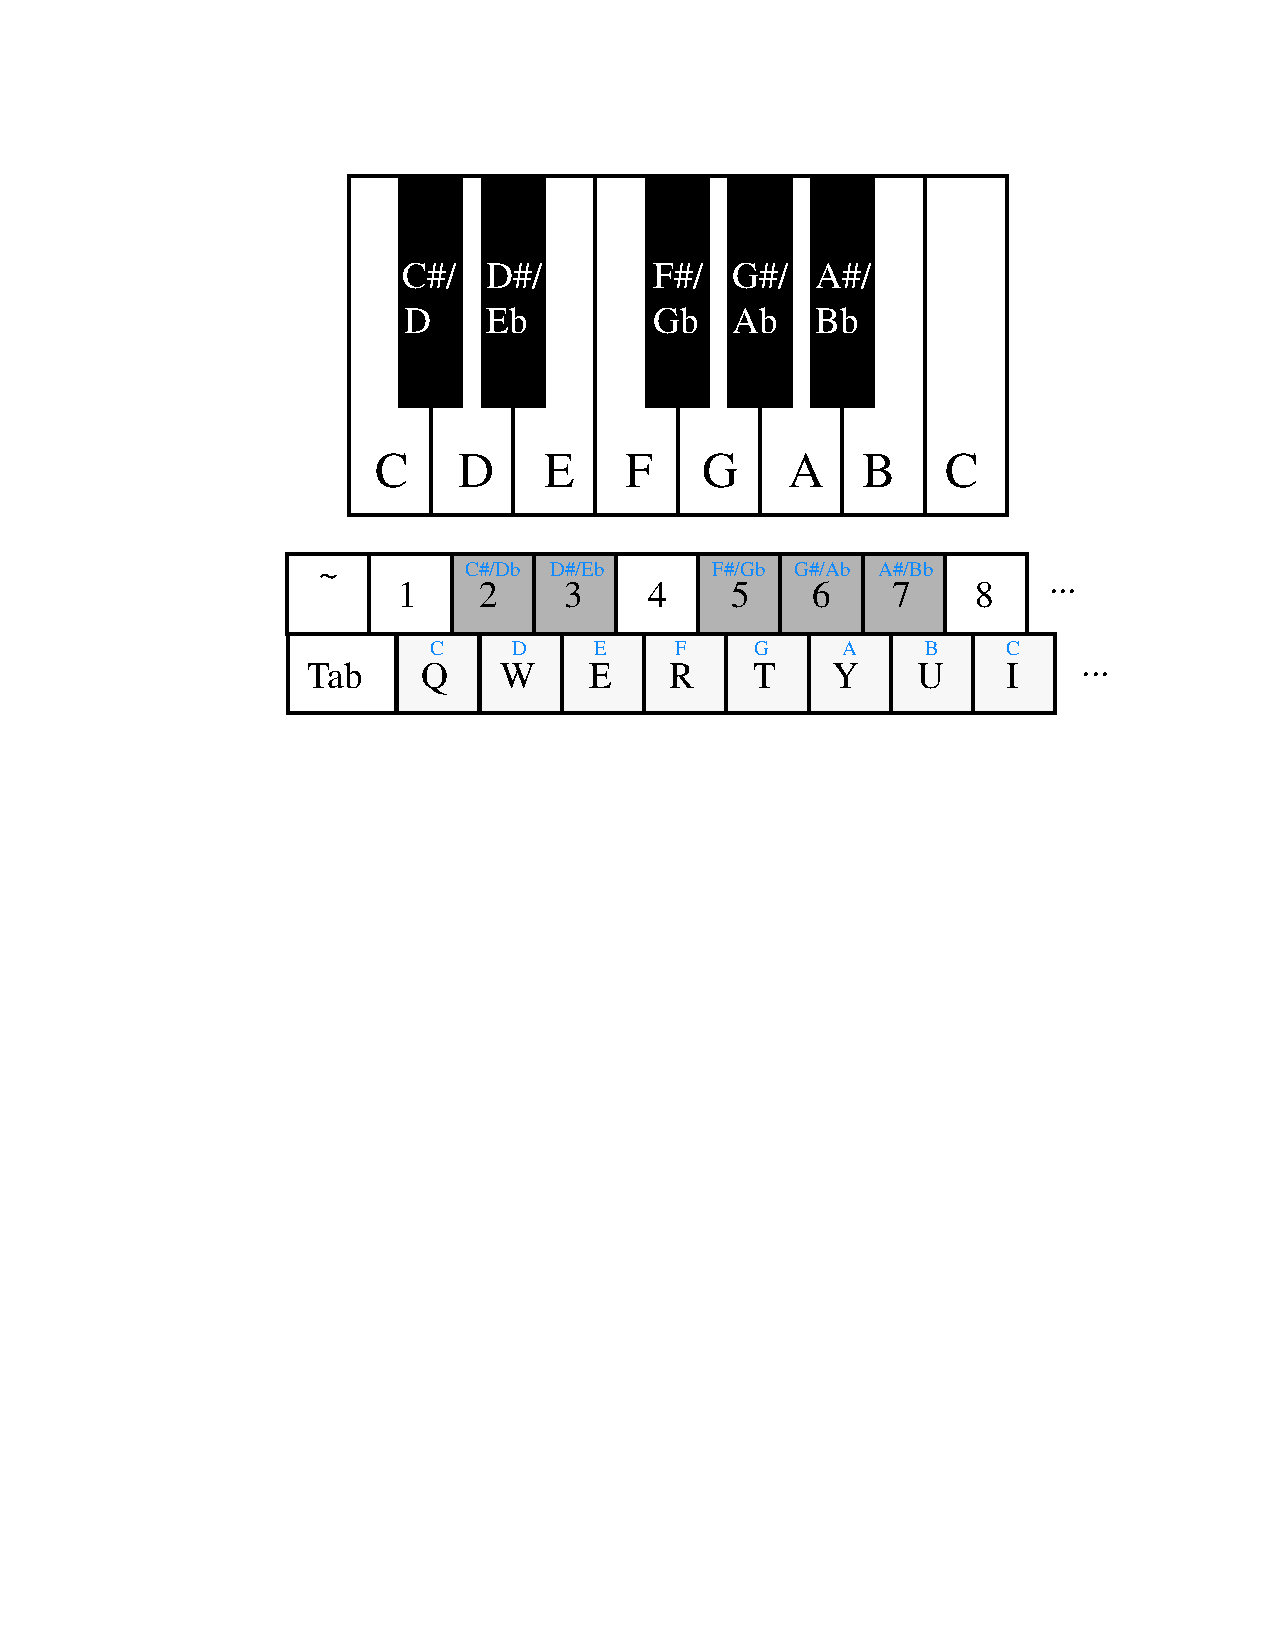
\includegraphics[scale=0.5]{figures/keyboard_layout.pdf}
   \end{center}
   \caption{The mapping from piano keys to keyboard keys.}
	\label{fig:keyboard_layout}
\end{figure}

~\\
\noindent
The audio thread can be created from within the main thread by using the
{\it Pthreads} application programming interface (API), which is included as part of Linux. 
To use this API in your code, you must include the \texttt{<pthread.h>} header file and
compile your code with the flag \texttt{-pthread} appended to your \texttt{gcc} command. 
Skeleton code for
using this API is shown in Figure~\ref{fig:pthread_code}. In this code, the main program
loops to read the USB keyboard, representing the piano keys (tones). When a key is pressed, the
main program adjusts the volume of the corresponding tone in the \texttt{tone\_volume} array.
The audio thread loops to read the \texttt{tone\_volume} array, and creates a sinusoid for
each tone that is currently being played.

~\\
\noindent
The audio thread is similar to the code from
Part~II, because it has to create, and possibly sum together, sinusoids corresponding to
each tone. You may want to structure your audio thread so that it, in addition to generating
the tone-sounds, slowly reduces the volume of each tone depending on whether or not the
key for this tone is still being pressed. This approach simulates the way in which actual piano
keys behave.

\lstset{language=C,numbers=left}
\begin{figure}[H]
\begin{center}
\begin{minipage}[t]{14 cm}
\begin{lstlisting}
#include <stdio.h>
#include <fcntl.h>
#include <linux/input.h>

#define KEY_RELEASED 0
#define KEY_PRESSED 1

int main (int argc, char *argv[])
{
	struct input_event ev;
	int fd, event_size = sizeof (struct input_event);

	// Get the keyboard device 
	if (argv[1] == NULL){
	    printf("Specify the path to the keyboard device ex. /dev/input/by-id/HP-KEYBOARD");
	    return -1;
	}
 
	// Open keyboard device
	if ((fd = open (argv[1], O_RDONLY |$\mid$| O_NONBLOCK)) == -1){
	    printf ("Could not open %s\n", argv[1]);
	    return -1;
	}

	while (1){
	    // Read keyboard
	    if (read (fd, &ev, event_size) < event_size){
	        // No event
	        continue;
	    }
	    if (ev.type == EV_KEY && ev.value == KEY_PRESSED){
	        printf("Pressed key: 0x%04x\n", (int)ev.code);
	    } else if (ev.type == EV_KEY && ev.value == KEY_RELEASED){
	        printf("Released key: 0x%04x\n", (int)ev.code);
	    }
	}
	close(fd);
	return 0;
}
\end{lstlisting}
\end{minipage}
\end{center}
\vspace{-0.33in}\caption{Reading keyboard input.}
\label{fig:keyboard_code}
\end{figure}

Important lines of code in Figure~\ref{fig:pthread_code} are discussed below:

\begin{itemize}
\item Lines \ref{line:audio_begin} - \ref{line:audio_end} implement the function that is
executed in the audio thread. As shown, this function has to have the type \texttt{void *}.
\item Line \ref{line:check_cancel} calls the function \texttt{pthread\_testcancel}, which checks
if the thread has been cancelled by the main thread. If it has been cancelled, the
audio thread will halt execution at this point and terminate.
\item Line \ref{line:create} calls \texttt{pthread\_create} to create the audio thread. The
arguments are:
\begin{itemize}
\item \&{\it pid}: the variable in which the {\it thread id}, a unique integer identifier for the 
thread, will be stored.
\item NULL: a pointer to an {\it attributes} structure can be passed to specify some
properties of the spawned thread. A NULL argument causes the thread to use default attributes.
\item \&{\it audio\_thread}: a pointer to the \texttt{audio\_thread} function
that we want to execute in the audio thread.
\item NULL: This argument can be any value, and in general practice would be a pointer to
a structure containing all of the variables (arguments) that we want to pass into
the thread. In our case the variables that are needed by the \texttt{audio\_thread}, such
as \texttt{tone\_volume}, are global variables, which do not need to be passed to the thread
as arguments.
\end{itemize}
\item Line \ref{line:cancel}: the call to the function \texttt{pthread\_cancel} sends a
\textit{cancel} signal to the thread, which causes the audio thread to stop executing when
it reaches \texttt{pthread\_testcancel}.
\item Line \ref{line:join}: the \texttt{pthread\_join} function forces the main thread to wait
until the audio thread has been terminated before continuing past this point. 
\end{itemize}

\lstset{language=C,numbers=left,escapechar=|}
\begin{figure}[H]
\begin{center}
\begin{minipage}[t]{14.75 cm}
\begin{lstlisting}
#include <math.h>
#include <linux/input.h>
#include <pthread.h>
|$\ldots$| other include statements

int tone_volume[13];
|$\ldots$| other global variables (not shown)

|\label{line:audio_begin}|void *audio_thread( ){
	int i;
	while(1){
	    // Check if this thread has been cancelled.
	    // If it was, the thread will halt at this point.
	    |\label{line:check_cancel}|pthread_testcancel();
	    |$\ldots$|
	    // Code for writing to the audio port.
	    for (i=0; i < NUM_OF_TONES; i++){
	        |$\ldots$| tone_volume[i] |$\ldots$|
	    }
	    |$\ldots$|
	}
|\label{line:audio_end}|}

int main (int argc, char *argv[])
{
	int err;
	pthread_t tid;
	|$\ldots$|

	// Spawn the audio thread.
	|\label{line:create}|if ((err = pthread_create(&tid, NULL, &audio_thread, NULL)) != 0)
	    printf("pthread_create failed:[%s]\n", strerror(err));

	while (1){
	    // Read keyboard and adjust tone_volume[].
	    |$\ldots$|
	}
	// Cancel the audio thread.
	|\label{line:cancel}|pthread_cancel(tid);
	// Wait until audio thread terminates.
	|\label{line:join}|pthread_join(tid, NULL);

	return 0;
}
\end{lstlisting}
\end{minipage}
\end{center}
\vspace{-0.33in}\caption{Spawning the audio thread.}
\label{fig:pthread_code}
\end{figure}

\newpage
\noindent
{\bf Using a Mutex}

~\\
\noindent
If multiple threads in a program need to modify a single, shared, variable it is useful to 
synchronize access to that variable by using a {\it mutex}. For example, 
Figure~\ref{fig:mutex} indicates how a mutex can be used to synchronize writes to the 
\texttt{tone\_volume} array by both the main and audio threads. In this code the mutex is
declared as a global variable, and then {\it locked/unlocked} by each thread. The main
thread writes to \texttt{tone\_volume} when a piano key is pressed, and the audio
thread gradually reduces the volume of a tone depending on whether the key is still pressed.
More details about mutexes and pthreads can be found by searching on the Internet.

~\\
\noindent
Perform the following:

\begin{enumerate}
\item Make a new folder to hold your C source code. Augment your code from Part II so that
it uses two threads as illustrated in Figure~\ref{fig:pthread_code}. In your main thread
open the appropriate keyboard device in the folder {\it /dev/input}, to provide your piano keys.
When you press a key the tone should immediately sound, and then gradually fade away as
indicated in Figure~\ref{fig:mutex}.
\item Compile your program using a command such as \texttt{gcc -o part3 part3.c -lm -pthread}
\end{enumerate}

\lstset{language=C,numbers=none,escapechar=|}
\begin{figure}[H]
\begin{center}
\begin{minipage}[t]{14.75 cm}
\begin{lstlisting}
|$\ldots$|
int tone_volume[13];
pthread_mutex_t mutex_tone_volume;  // mutex for main and audio_thread
|$\ldots$|

void *audio_thread( ){
	|$\ldots$| code |for| creating and outputting waveforms not shown
	// Fade the tones
	for (j = 0; j < 13; j++){
		if (tone_volume[j] > |$\ldots$|){
			pthread_mutex_lock (&mutex_tone_volume);	// lock the mutex
			tone_volume[j] *= tone_fade_factor[j];
			pthread_mutex_unlock (&mutex_tone_volume);	// unlock the mutex
		}
	}
}

int main (int argc, char *argv[])
{
	|$\ldots$|
	pthread_t tid;
	if ((err = pthread_create(&tid, NULL, &audio_thread, NULL)) != 0)
		printf("pthread_create failed:[%s]\n", strerror(err));
	while (1){
		// Read keyboard and adjust tone_volume[].
		|$\ldots$|
		pthread_mutex_lock (&mutex_tone_volume);	// lock the mutex
		tone_volume[tone_index] = |$\ldots$|
		pthread_mutex_unlock (&mutex_tone_volume);	// unlock the mutex
		tone_fade_factor[tone_index] = |$\ldots$|
	}
	|$\ldots$|
}
\end{lstlisting}
\end{minipage}
\end{center}
\vspace{-0.33in}\caption{Using a mutex to control access to the \texttt{tone\_volume} array.}
\label{fig:mutex}
\end{figure}

\noindent
\section*{Part IV}

\noindent
Figure~\ref{fig:sinewaves} shows two sinusoidal waveforms. The top waveform represents
middle C, also known as tone C4, which has the frequency 261.626~Hz, and the bottom
waveform represents tone C5, which has the frequency 523.251~Hz. For this part of the
exercise you are to augment your piano code such that it can draw waveforms on a 
display corresponding to the sound that is currently being played. If a single tone is
being played, then your waveform will be a sine wave, like the ones depicted in
Figure~\ref{fig:sinewaves}, but if a chord is being played then
you would display the waveform represented by the sum of the individual tones.
Rather than drawing waveforms continuously, just draw a few cycles whenever the piano
``keys'' are pressed, or released. 

\begin{figure}[H]
   \begin{center}
			  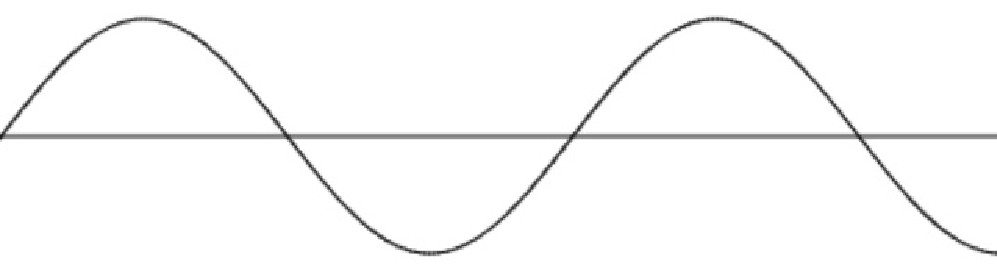
\includegraphics[scale=0.67]{figures/middleC.pdf}
			  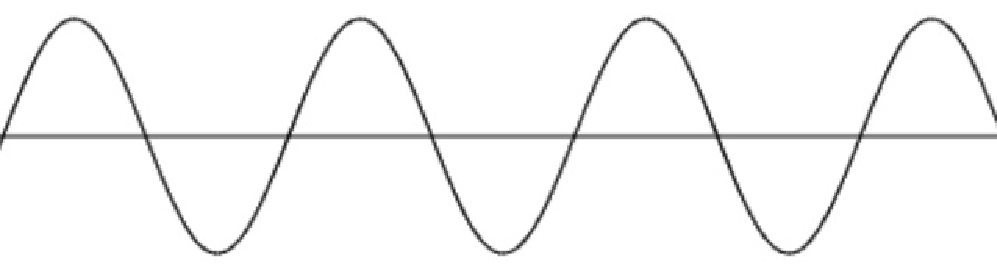
\includegraphics[scale=0.67]{figures/nextC.pdf}
   \end{center}
   \caption{Sine waves for tones C4 and C5.}
	\label{fig:sinewaves}
\end{figure}

~\\
\noindent
You can display waveforms using the VGA output of your DE-series board. At the sampling rate 
of 8000 samples/second, there are $8000 \div 261.626 \simeq 30.5$ samples per cycle for 
tone C4. Given that there are 320 columns in the VGA display for the DE1-SoC Computer, it 
is easy to display about $320 \div 30.5 \simeq 10.5$ cycles of this waveform. Using the same 
approach you could display about $320 \div (8000 \div 523.251) \simeq 21$ cycles of tone C5.
If you are using the DE10-Standard board, then you may want to use the LCD display
provided on the board. In this case you may display fewer cycles of the waveform, because 
there are 128 columns in the display rather than 320.

~\\
\noindent
Perform the following:

\begin{enumerate}
\item Make a new folder to hold your C source code. Augment your code from Part III to
create a third thread called {\it video\_thread}. In this new thread you should provide
the code for drawing waveforms on the display. To communicate with the VGA controller
in the DE1-SoC Computer you can use a character device driver. Such a driver can be found
in {\it /home/root/Linux\_Libraries/drivers/video.ko}, and is described in the tutorial 
{\it Using Linux on DE-series Boards}. If you are using the LCD display on the
DE10-Standard board, then the {\it LCD.ko} driver can be used instead. 

Since there are now three threads in your program and only two CPU cores in the DE1-SoC
Computer, the threads must share the processor cores. It is important to ensure that
the audio thread always has access to a CPU core so that the audio-port's {\it Write} FIFOs
do not become empty. One approach for handling the three threads is to assign
the main and video threads to one CPU core, while assigning the audio thread to the other
core. Figure~\ref{fig:cpucore} provides a function that can be called by a thread to
assign it to a specific CPU core. In the main and video threads you could call 
\texttt{set\_processor\_affinity(0)}, assigning these threads to CPU core 0, 
and in the audio thread \texttt{set\_processor\_affinity(1)}, assigning 
this thread to CPU core 1. To use the \texttt{CPU\_ZERO} and \texttt{CPU\_SET} macros in 
Figure~\ref{fig:cpucore} you have to define \texttt{\_GNU\_SOURCE} and include the header
file \texttt{<sched.h>}, as shown in the code.
\item Compile and test your program. Check that tones and chords that are played on the
piano sound the same as they did in Part III, confirming that your threads are working
properly. Check that your video thread draws appropriate waveforms for each tone and chord
played on the piano.
\end{enumerate}

\lstset{language=C,numbers=none,escapechar=|}
\begin{figure}[H]
\begin{center}
\begin{minipage}[t]{14.75 cm}
\begin{lstlisting}
#define _GNU_SOURCE 
#include <pthread.h>
#include <sched.h>
|$\ldots$|
// Set the current thread's affinity to the core specified
int set_processor_affinity(unsigned int core){
	cpu_set_t cpuset;
	pthread_t current_thread = pthread_self(); 
    
	if (core >= sysconf(_SC_NPROCESSORS_ONLN)){
		printf("CPU Core %d does not exist!\n", core);
		return -1;
	}
    
	// Zero out the cpuset mask
	CPU_ZERO(&cpuset);
	// Set the mask bit for specified core
	CPU_SET(core, &cpuset);
    
	return pthread_setaffinity_np(current_thread, sizeof(cpu_set_t), &cpuset); 
}

\end{lstlisting}
\end{minipage}
\end{center}
\vspace{-0.33in}\caption{Assigning a thread to a CPU core.}
\label{fig:cpucore}
\end{figure}

\noindent
\section*{Part V}

\noindent
For this part you are to further enhance your code from Part IV so that it is possible to
record, for later playback, music that is played on the piano.

~\\
\noindent
Perform the following:

\begin{enumerate}
\item Augment your source code from Part IV to create a data structure that can be used to
store recorded music. In this data structure you should record when each piano key is
pressed, and when it is released. Both the recoding process and playback should be handled
by the main thread in your program. To keep track of time you can use a timer, like the
{\it stopwatch} that was discussed in Laboratory Exercise 4, Part 2. This {\it stopwatch}
provides a character device driver via the file {\it /dev/stopwatch}, which provides the current
time when read, and can be written to set the time. The {\it stopwatch} decrements at a
rate of $1/100^{th}$ seconds, which is sufficiently accurate for our purposes.
\item You should start recording notes when the user presses the pushbutton KEY$_0$ in the
DE1-SoC Computer. Pressing this button again should stop the recording. The recording should be
played back when KEY$_1$ is pressed. You should illuminate LEDR$_0$ while recording
music, and LEDR$_1$ during playback. In addition to using the {\it stopwatch} to measure
time during recording, you can also use it to control the time between notes during
playback. Show the {\it stopwatch} time on the seven-segment displays HEX5 - HEX0.
\item You can use character devices drivers to communicate with the KEY pushbuttons and LEDR
lights. Suitable drivers are available in the directory
{\it /home/root/Linux\_Libraries/drivers}.
\item Compile and test your program. During both recording and playback of music you
should be able to hear the music being played and see the corresponding waveforms on the
VGA display.
\end{enumerate}

\newpage
\noindent
\section*{Part VI}

\noindent
So far in this exercise you have used memory-mapped I/O to communicate with the audio-out
port. For this part, you are to modify your approach so that your program communicates with
the audio port through a character device driver.

~\\
\noindent
Perform the following:

\begin{enumerate}
\item A Linux character device driver for the audio port is available in 
{\it /home/root/Linux\_Libraries/drivers/audio.ko}. The interface to this driver, which uses the
file {\it /dev/IntelFPGAUP/audio}, is described in the tutorial {\it Using Linux on 
DE-series Boards}. You can write the following commands to the driver: \texttt{init}, 
which clears the audio 
FIFOs, \texttt{waitw}, which checks the depths of the {\it Write} FIFOs and waits for some 
free space, \texttt{left data}, and \texttt{right data}. These last two commands write the 
supplied data, specified as a signed integer, into the audio-port's left and right data 
registers. After inserting the audio driver into the Linux kernel, you can obtain a listing of 
its commands by executing the Linux command \texttt{echo -$\,$- > /dev/IntelFPGAUP/audio}.
\item Change your piano source code so that it uses the audio character device driver
instead of using memory-mapped I/O. Compile the modified program and test to ensure that
it works the same as it did in Part V.
\end{enumerate}

~\\

\vskip 0.8in
\noindent
\newpage
%%%%%%%%%%%%%%%%%%%%%%%%%%%%%%%%%%%%%%%%
%%% FPGAcademy Copyright Information %%%
%%%%%%%%%%%%%%%%%%%%%%%%%%%%%%%%%%%%%%%%

%Always put the copyright on a new page (clear page), with some vertical space from top
\clearpage
\vspace{1in}

\noindent

Copyright {\copyright} FPGAcademy.org. All rights reserved. FPGAcademy and the 
FPGAcademy logo are trademarks of FPGAcademy.org.  This document is provided 
"as is", without warranty of any kind, express or implied, including but not 
limited to the warranties of merchantability, fitness for a particular purpose 
and noninfringement. In no event shall the authors or copyright holders be 
liable for any claim, damages or other liability, whether in an action of 
contract, tort or otherwise, arising from, out of or in connection with the 
document or the use or other dealings in the document.
~\\
~\\
**Other names and brands may be claimed as the property of others.



\end{document}
